% Author: Izaak Neutelings (September 2020)
% Inspiration: https://tex.stackexchange.com/questions/25531/adding-underbrace-in-tikz
\documentclass[border=3pt,tikz]{standalone}
\usepackage{physics}
\usepackage{ifthen}
\usepackage{tikz}
\usetikzlibrary{patterns,snakes}
\tikzset{>=latex} % for LaTeX arrow head

\colorlet{myred}{red!65!black}
\tikzstyle{ground}=[preaction={fill,top color=black!10,bottom color=black!5,shading angle=20},
                    pattern=north east lines,draw=none,minimum width=0.3,minimum height=0.6]
\tikzstyle{mass}=[line width=0.6,red!30!black,fill=red!40!black!10,rounded corners=1,
                  top color=red!40!black!20,bottom color=red!40!black!10,shading angle=20]
\tikzstyle{rope}=[brown!70!black,line width=2] %very thick
\def\rope#1{ \draw[black,line width=2.3] #1; \draw[rope] #1; }

% FORCES SWITCH
\tikzstyle{force}=[->,myred,thick,line cap=round]
\newcommand{\vbF}{\vb{F}}
\newcommand{\vbT}{\vb{T}}
\newboolean{showforces}
\setboolean{showforces}{true}

\begin{document}


% VERTICAL ceiling
\def\h{0.6} % mass height
\def\w{0.7} % mass width
\begin{tikzpicture}
  \def\W{2.0} % ground width
  \def\D{0.2} % ground depth
  \def\H{3.0} % ground depth
  \def\y{0.5*\H} % mass y coordinate
  \rope{(0,\H) -- (0,\y)}
  \draw[ground] (-\W/2,\H) rectangle++ (\W,\D);
  \draw (-\W/2,\H) --++ (\W,0);
  \draw[mass] (-\w/2,\y) rectangle++ (\w,\h) node[midway] {$m$};
  
  % FORCES
  \ifthenelse{\boolean{showforces}}{
    \draw[force] (-0.3*\w,\y+0.9*\h) --++ (0, 1.0*\h) node[left=-1] {$\vbT$};
    \draw[force] (0.35*\w,\y+0.4*\h) --++ (0,-1.0*\h) node[below=-3] {$-mg\vu{y}$};
  }{}
  
\end{tikzpicture}


% VERTICAL rope
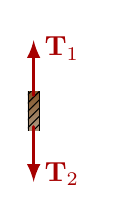
\begin{tikzpicture}
  \def\h{0.5}
  \def\w{0.15}
  \draw[preaction={fill,top color=brown!70!black,bottom color=brown!60!black!60,shading angle=20},
        pattern=north east lines,draw=none,minimum width=0.3,minimum height=0.6]
    (-\w/2,0) rectangle++ (\w,\h);
  \draw (-0.46*\w,0) --++ (0,\h) (\w/2,0) --++ (0,\h);
  \draw[force,very thick] (0,0.9*\h) --++ (0, 1.4*\h) node[below=3,right=0] {$\vbT_1$};
  \draw[force,very thick] (0,0.1*\h) --++ (0,-1.4*\h) node[above=3,right=0] {$\vbT_2$};
\end{tikzpicture}


% VERTICAL ceiling 2
\begin{tikzpicture}
  \def\W{2.0} % ground width
  \def\D{0.2} % ground depth
  \def\H{1.5} % ground depth
  \def\y{0} % mass y coordinate
  \coordinate (M) at (0,0);
  \rope{(-0.4*\W,1.05*\H) -- (M) -- (0.4*\W,1.05*\H)}
  \draw[ground] (-\W/2,\H) rectangle++ (\W,\D);
  \draw (-\W/2,\H) --++ (\W,0);
  \draw[mass] (M)++(-\w/2,0) rectangle++ (\w,-\h) node[midway] {$m$};
\end{tikzpicture}


% VERTICAL ceiling 3
\begin{tikzpicture}
  \def\W{2.0} % ground width
  \def\D{0.2} % ground depth
  \def\H{1.5} % ground depth
  \coordinate (M) at (0,0);
  \rope{(-0.4*\W,1.05*\H) -- (0,0.4*\H) coordinate (R) -- (0.4*\W,1.05*\H)
    (R) -- (M);}
  \draw[ground] (-\W/2,\H) rectangle++ (\W,\D);
  \draw (-\W/2,\H) --++ (\W,0);
  \draw[mass] (M)++(-\w/2,0) rectangle++ (\w,-\h) node[midway] {$m$};
\end{tikzpicture}



% HORIZONTAL ground - lift
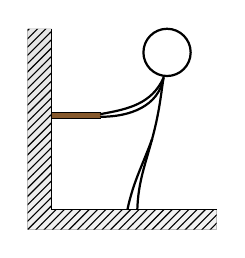
\begin{tikzpicture}
  \def\WH{2.3}  % wall height
  \def\WT{0.3}  % wall thickness
  \def\GW{2.1}  % ground width
  \def\GD{0.25} % ground depth
  \def\h{0.6}   % mass height
  \def\w{0.7}   % mass width
  \def\H{2.0}   % human height
  \def\mx{0.5*\GW} % mass x coordinate
  
  % SETUP
  \rope{(0,0.6*\H) --++ (0.3*\GW,0) coordinate (RH)}
  \draw[ground] (0,0) -- (0,\WH) --++ (-\WT,0) --++ (0,-\WH-\GD) --++
                (\WT+\GW,0) -- (\GW,0) -- cycle;
  \draw (0,\WH) -- (0,0) -- (\GW,0);
  
  % PERSON
  \draw[thick] (0.7*\GW,\H) circle (0.3) coordinate (H);
  \draw[thick] (H)++(-98:0.3) coordinate (N) to[out=-98,in=75]++ (-0.07*\GW,-0.40*\H) coordinate (P);
  \draw[thick,line cap=round] (N)++(-98:0.03) to[out=-115,in=10] ([yshift=0.5]RH);
  \draw[thick,line cap=round] (N)++(-98:0.03) to[out=-100,in=0] ([yshift=-0.5]RH);
  \draw[thick] (P) to[out=-110,in=78] (0.46*\GW,0);
  \draw[thick] (P) to[out=-105,in=88] (0.52*\GW,0);
  
\end{tikzpicture}


\end{document}